\documentclass[a4paper,onecolumn,10pt]{article}
\usepackage[polish]{babel}
\usepackage[utf8]{inputenc}
\usepackage[T1]{fontenc}
\usepackage[left=2.1cm,right=2.1cm]{geometry}
\usepackage[dvipsnames]{xcolor}
\usepackage{amsmath,calc,indentfirst,fancyhdr,amsfonts,graphicx,epstopdf,caption, mathcomp, subcaption,wrapfig, siunitx,pbox,float,algorithm}
\usepackage[noend]{algpseudocode}


\makeatletter
\def\BState{\State\hskip-\ALG@thistlm}
\renewcommand{\ALG@name}{Algorytm}
\makeatother

\renewcommand{\baselinestretch}{1.1}	 % odstep miedzy liniami
\addto\captionspolish{\renewcommand{\figurename}{Wykres}} % zmiana podpisu pod obrazkami, zamiast "Rysunek" bedzie "Wykres"
\newcommand{\NN}{\mathbb{N}}			 % makro do znaku liczb naturalnych

\newcommand{\R}[1]{\textcolor{red}{#1}}  % makro do polecenia z parametrami - tutaj 1 parametr
\newcommand{\G}[1]{\textcolor{green}{#1}} 
\newcommand{\B}[1]{\textcolor{RoyalBlue}{#1}} 
% kolorowanie {\B{argument}}

\newcommand{\PICTURES}{} % szybsza kompilacja dzieki stalej "usuwajacej" obrazki
						 % zakomentowanie \PICTURES powoduje znikniecie obrazkow

\pagestyle{fancy} % formatuj caly dokument
\fancyhead{}
\fancyfoot{}
\renewcommand{\headrulewidth}{0pt}
\fancyfoot[R]{\thepage} % dla stron poza tytulowa nr w prawym dolnym rogu

\fancypagestyle{plain}{ % dla strony tytulowej nr w prawym dolnym rogu
	
	\renewcommand{\headrulewidth}{0pt}
	\fancyhf{}
	\fancyfoot[R]{\thepage}
}
% 17 linia w preamble.tex

\renewcommand{\arraystretch}{1.2}

\title{\Large\vspace{-2.5cm}{\Huge S}PRAWOZDANIE - LABORATORIUM NR {\Huge8}\\
	\textbf{Interpolacja funkcjami sklejanymi w bazie} } 
\date{\Large25 kwietnia 2019}
\author{\Large Marek Kiełtyka}

\begin{document}
\maketitle

\vspace{-1.2cm}\section{Wstęp}

\subsection{Interpolacja funkcjami sklejanymi}

W przedziale [a, b] istnieje $n+1$ punktów takich, że:
\begin{equation} 
\label{wezly}
a = x_0 < x_1 < x_2 < \dots < x_{n-2} < x_{n-1} < x_{n} = b
\end{equation}
Powyższe punkty reprezentują podział przedziału [a,b] na $n$ podprzedziałów 
[$x_i$,~$x_{i+1}$].
Funkcja $s(x)$ określona na przedziale [a, b] to \textbf{funkcja sklejana} stopnia $m$ przy założeniach:
\begin{itemize}
	\item $m \geq 1$
	\item $s(x)$ jest wielomianem stopnia maksymalnie $m$ na każdym podprzedziale $[x_i$; $x_{i+1}], i=0,1,...,n-1$
	\item  $s(x) \in C^{m}$
\end{itemize}
Punkty $x_j$ nazywamy węzłami funkcji sklejanej. Funkcja $s(x)$ występuje więc w każdym przedziale w postaci wielomianu, który można przedstawić wzorem:
\begin{equation}
s_i(x) = c_{im}x^m + c_{im-1}x^{m-1} + \cdots + c_{i1}x + c_{i0}, \qquad x \in (x_i; x_{i+1}).
\end{equation}
Funkcja interpolująca jest kombinacją liniową elementów bazy \{$s_i(x)$\}
\begin{equation}
s(x) = \sum_{i=0}^{n-1} c_i s_i (x) \quad x \in [a, b].
\end{equation}

\subsection{Przepis}

Przy założeniu o równoodległych węzłach oraz bazie złożonej z funkcji 
\begin{equation}
\phi_i^3(x), i = -1, 0, 1, \dots, n+1
\end{equation}
można po przesunięciu indeksu zapisać funkcję interpolującą w postaci
\begin{equation}
s(x) = \sum_{i = 0}^{n + 1}c_i\phi_i^3(x), x\in [x_{min}, x_{max}]
\label{es}
\end{equation}
gdzie
\begin{equation}
	\phi_i^3(x) = \frac{1}{h^3} 
	\begin{cases}
		(x - x_{i-2})^3 &x\in[x_{i-2},x_{i-1})\\
		h^3 + 3h^2(x-x_{i-1}) + 3h(x-x_{i-1})^2 -3(x-x_{i-1})^3 &x\in[x_{i-1},x_{i})\\
		h^3 + 3h^2(x_{i+1}-x) + 3h(x_{i+1}-x)^2 -3(x_{i+1}-x)^3&x\in[x_{i},x_{i+1}) \\
		(x_{i+2}-x)^3 &x\in[x_{i+1},x_{i+2})\\
		0&x\notin[x_{-3},x_{i+3}]
	\end{cases}
	\label{przepis}
\end{equation}
Tak określone sklejki kubiczne w teorii dają najlepsze rezultaty, toteż dokonano weryfikacji tego stwierdzenia.

\section{Zadanie do wykonania}

\subsection{Opis problemu}

Celem laboratorium była interpolacja funkcji 
\begin{equation}
f_1(x) = \frac{1}{1 + x^2} \mbox{ dla } n = 5, 6, 10, 20
\label{f1}
\end{equation}
oraz
\begin{equation}
f_2(x) = cos(2x) \mbox{ dla } n = 6, 7, 14
\label{f2}
\end{equation}
(gdzie $ n $ - liczba węzłów) w przedziale $ x\in [-5,5] $ po uprzednim rozwiązaniu układu równań postaci
\begin{equation} 
\label{uklad}
\begin{bmatrix}
4 & 2 & &  &  &  \\
1 & 4 & 1 &  & 0 &  \\
 & 1 & 4 & \ddots &  &  \\
 & &\ddots & \ddots & \ddots &\\
 & 0 &  & 1 & 4 & 1 \\
 &  &  & & 2 & 4 \\
\end{bmatrix}
\begin{bmatrix}
c_1 \\
c_2 \\
c_3 \\
\vdots \\
c_{n-1} \\
c_{n}
\end{bmatrix}
=
\begin{bmatrix}
y_1 + \frac{h}{3}\alpha \\
y_2 \\
\vdots \\
\vdots \\
y_{n-1} \\
y_{n} - \frac{h}{3}\beta
\end{bmatrix}
\end{equation}
\begin{alignat*}{3}
\alpha&= \frac{df(x)}{dx}, x = x_{min}\\
\beta &= \frac{df(x)}{dx}, x = x_{max}
\end{alignat*}
Dla każdego przypadku należało sporządzić wykresy funkcji interpolowanej i interpolującej na jednym rysunku.

\subsection{Wyniki}

Korzystając z alokacji macierzy i wektorów w stylu biblioteki \textit{Numerical Recipes} oraz jednej z jej funkcji do rozwiązywania układów równań liniowych (w tym przypadku była to \textit{gaussj}) rozpatrzono siedem przypadków, zgodnie z zadanymi funkcjami (\ref{f1}) oraz (\ref{f2}). Do przybliżania kolejnych wartości używano przepisów (\ref{es}) oraz (\ref{przepis}). Wyniki zaprezentowano poniżej.
\newpage
\begin{figure}[h!]
	\begin{tabular}{cc}
		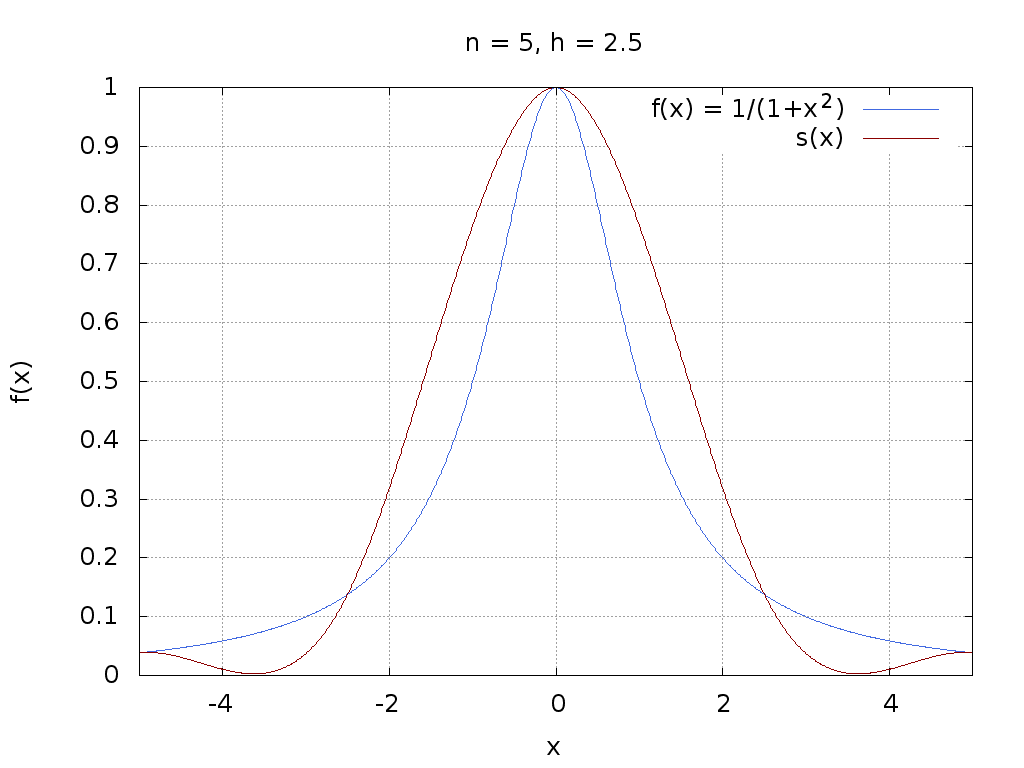
\includegraphics[width=81mm]{f1n5.png} &   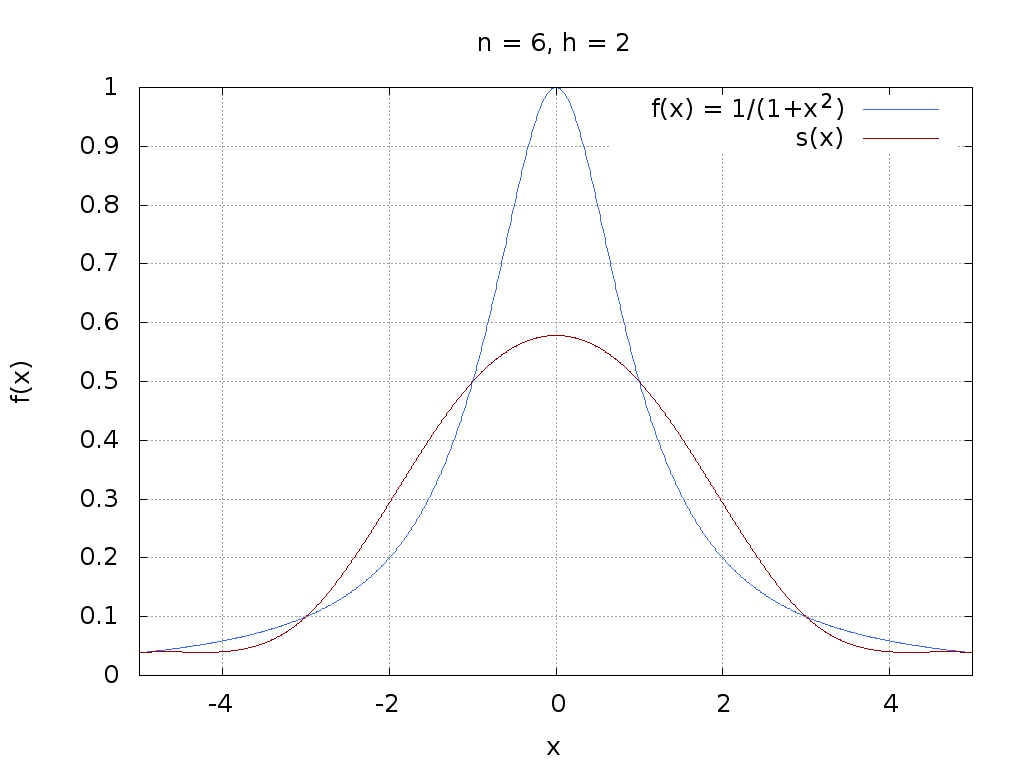
\includegraphics[width=81mm]{f1n6.png} \\
		[6pt]
		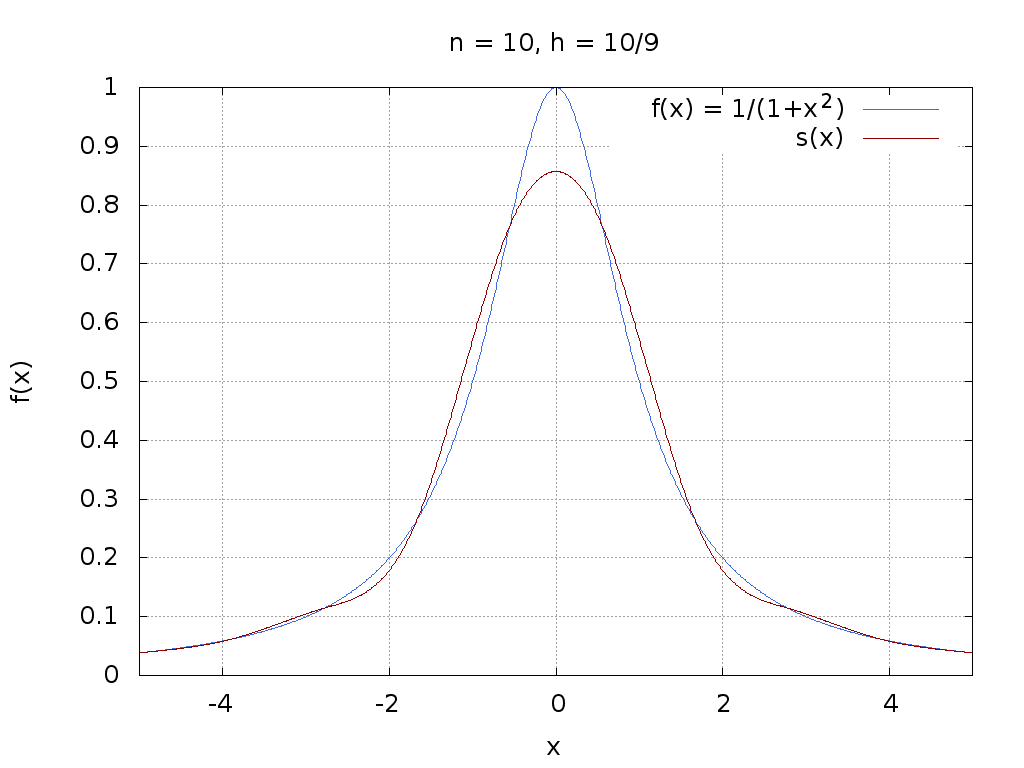
\includegraphics[width=81mm]{f1n10.png} &   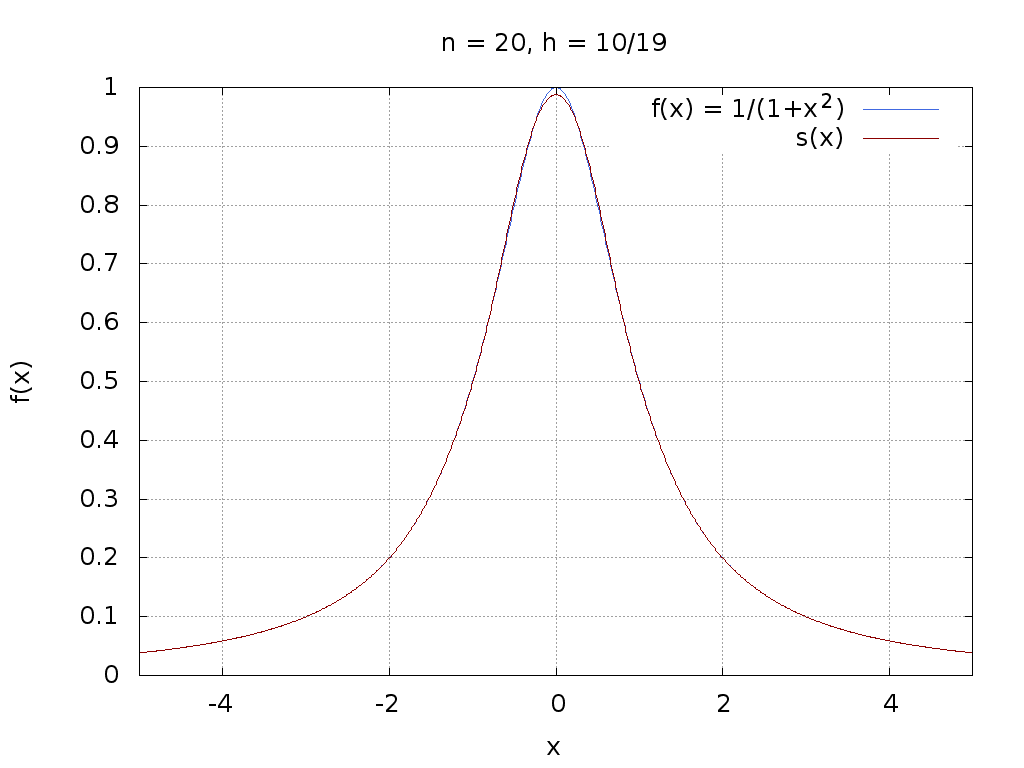
\includegraphics[width=81mm]{f1n20.png} \\
		[6pt]
	\end{tabular}
	\caption{Wyniki interpolacji funkcji $ f_1(x) = \frac{1}{1 + x^2} $ kubicznymi funkcjami sklejanymi w bazie dla $ n $ węzłów.}
	\label{pierwsza} 
\end{figure}
\begin{figure}[h!]
	\begin{tabular}{cc}
		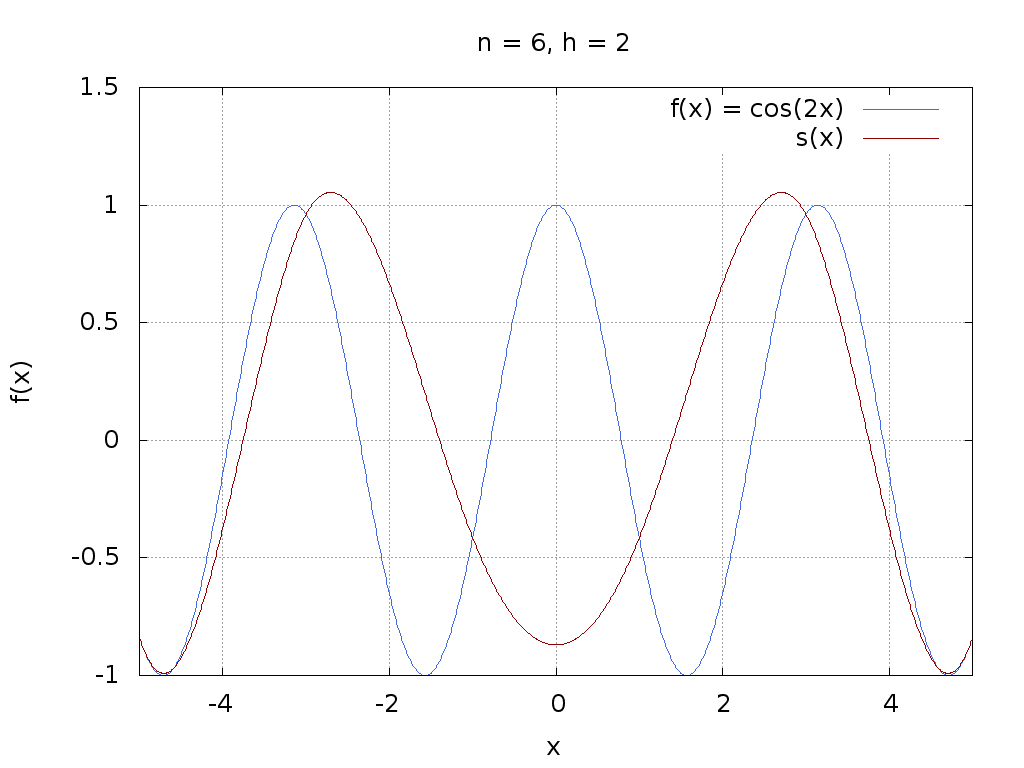
\includegraphics[width=81mm]{f2n6.png} &   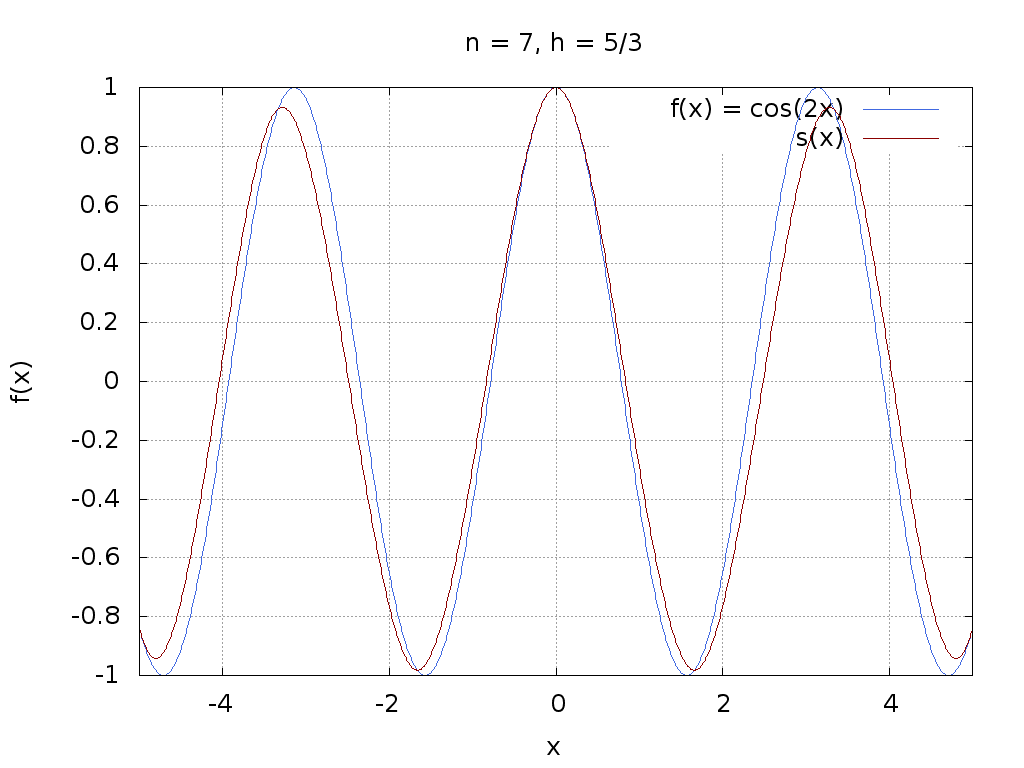
\includegraphics[width=81mm]{f2n7.png} \\
[6pt]
		\multicolumn{2}{c}{\centering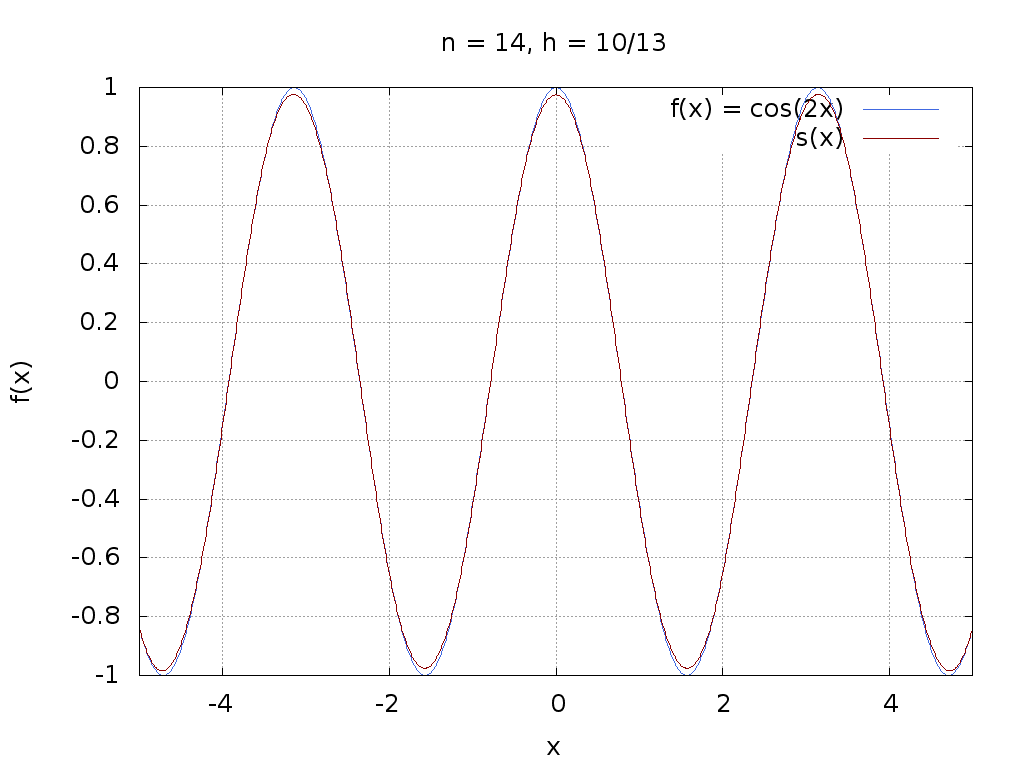
\includegraphics[width=81mm]{f2n14.png}}
	\end{tabular}
	\caption{Wyniki interpolacji funkcji $ f_2(x) = cos(2x) $ kubicznymi funkcjami sklejanymi w bazie dla $ n $ węzłów.}
	\label{druga}
\end{figure}

\newpage
\section{Wnioski}

Zaprezentowane wykresy dowodzą, iż interpolacja funkcjami sklejanymi w bazie jest efektywną czasowo metodą przybliżania wartości funkcji dla równoodległych węzłów. Dzięki niej uzyskano niemal pokrywające się wyniki dla 20 węzłów w przypadku funkcji hiperbolicznej i 14 dla trygonometrycznej. Jakość interpolacji sukcesywnie poprawiała się w miarę zwiększania ilości węzłów.

W przypadku innych metod dających tak dokładną interpolację przy niskiej ilości węzłów konieczne byłyby na przykład korekty ich położeń w celu uniknięcia efektu Rungego.

\end{document}